\documentclass[14pt,a4paper]{extarticle}
\usepackage{graphicx}
\usepackage{caption} 
\usepackage{hyperref}
\usepackage[T1]{fontenc}
\usepackage[utf8x]{inputenc}
\usepackage{pdfpages}
\usepackage{libertine}
\usepackage{listings}
\usepackage{xcolor}
\usepackage{enumitem}
\renewcommand{\thesection}{\arabic{section}}
\renewcommand{\familydefault}{\sfdefault}

\definecolor{stringgreen}{RGB}{100, 255, 100}

\lstdefinestyle{fish}{
	basicstyle=\small\ttfamily\color{black},
    keywordstyle=\color{blue},
	stringstyle=\medium\ttfamily\color{green},
    numberstyle=\tiny\color{gray},
    showstringspaces=false,
    tabsize=4,
	frame=single,
    breaklines=true,
    morekeywords={sudo,if,then,else,elif,fi,for,do,done,while,until,in},
}

\lstdefinestyle{json}{
	basicstyle=\small\ttfamily\color{black},
    showstringspaces=false,
    tabsize=2,
    breaklines=true,
}

\lstdefinestyle{sql}{
	basicstyle=\small\ttfamily\color{black},
    keywordstyle=\color{blue},
	stringstyle=\color{stringgreen},
    numberstyle=\tiny\color{gray},
    showstringspaces=false,
    tabsize=4,
    breaklines=true,
	language=SQL
}

\colorlet{punct}{red!60!black}
\definecolor{delim}{RGB}{20,105,176}
\colorlet{numb}{magenta!60!black}

\hypersetup{
    colorlinks=true,
    linkcolor=blue,
    filecolor=blue,      
    urlcolor=blue,
    pdfborder={0 0 0},
    linktocpage      
}

\begin{document}
	\begin{titlepage}
		\centering
		{\scshape\LARGE Big Data \par}
		\vspace{2.5cm}
		{\huge\bfseries Aggregations with MongoDB}
		\vfill
		{\normalsize von\par}
		{\normalsize Benjamin Ellmer (\textsc{S2210455012}) \par}
		\vspace{1cm}
		
\includegraphics[width=0.3\textheight]{images/logo.pdf} \par
		\vspace{1cm}
		{\large Mobile Computing Master \par}
		{\large FH Hagenberg \par}
		\vfill
		{\large \today\par}
	\end{titlepage}

	\section*{Step 1}
	\noindent \textbf{Install and start MongoDB using docker compose:}
	\begin{lstlisting}[style=fish]
git clone https://github.com/Digital-Media/fhooe-mongo-dock.git 
docker compose -f fhooe-mongo-dock/docker-compose.yml up -d
	\end{lstlisting}

	\noindent \textbf{Connect to the MongoDB shell in the container:}
	\begin{lstlisting}[style=fish]
docker exec -it mongodb /bin/bash -c "mongosh"
	\end{lstlisting}

	\noindent \textbf{Show and create database:}
	\begin{lstlisting}[style=fish]
show databases
use onlineshop
	\end{lstlisting}

	\noindent \textbf{Insert Data from exercise description:}
	\begin{lstlisting}[style=fish]
db.orders.insertMany([
	...
]);
	\end{lstlisting}

	\noindent \textbf{Find all rows of collection orders:}
	\begin{lstlisting}[style=fish]
db.orders.find({})
	\end{lstlisting}

	\newpage
	\section*{Step 2}
	\subsection*{My Summary}
	Map-reduce is a method of processing large volumes of data into useful aggregated results.
	MongoDB has a mapReduce command that performs map-reduce operations.
	In this process, MongoDB applies the map phase to each input document and emits key-value pairs, which are then condensed and aggregated using the reduce phase.
	The results are stored in a collection, and may also pass through a finalize function for further processing.
	Map-reduce functions in MongoDB are JavaScript-based and can perform arbitrary sorting and limiting before the map stage.
	They can also use custom JavaScript functions to provide flexibility to the operation, and can write results to a collection or return them inline.
	When writing to a collection, subsequent map-reduce operations can merge, replace or reduce new results with previous ones.

	\newpage

	\section*{Step 3}

	\noindent \textbf{Get sum of total sums:}
	\begin{lstlisting}[style=fish]
onlineshop> db.orders.aggregate([
	{
		$group: {
			_id: null, 
			totalSum: { $sum: "$total_sum" } 
		}
	}  
])
	\end{lstlisting}
	\noindent Output:
	\begin{lstlisting}[style=fish]
[ { _id: null, totalSum: 435 } ]
	\end{lstlisting}

	\vspace{1cm}

	\noindent \textbf{Get sum of qty * price per user:}
	\begin{lstlisting}[style=fish]
db.orders.aggregate([ 
	{ $unwind: "$items" }, 
	{ $group: { 
		_id: "$user_id", 
		sum:{ $sum: { $multiply: 
			[ "$items.price", "$items.qty"] 
		}}
	}}
])
	\end{lstlisting}
	\noindent Output:
	\begin{lstlisting}[style=fish]
[
  { _id: 2, sum: 125 },
  { _id: 4, sum: 155 },
  { _id: 1, sum: 95 },
  { _id: 3, sum: 60 }
]
	\end{lstlisting}

\newpage

	\noindent \textbf{Get sum of qty * price per user using mapReduce:}
\begin{lstlisting}[style=fish]
db.orders.mapReduce(
	function() { this.items.forEach(
		item => emit(this.user_id, item.qty * item.price)
	);},
	function(key, values) { return Array.sum(values); },
	{ out: { inline: 1 },
	  finalize: function(key, reducedValue) {
		return { _id: key, sum: reducedValue };
	  }
	}
)
\end{lstlisting}
\noindent Output:
\begin{lstlisting}[style=fish]
{
  results: [
    { _id: 1, value: { _id: 1, sum: 95 } },
    { _id: 4, value: { _id: 4, sum: 155 } },
    { _id: 2, value: { _id: 2, sum: 125 } },
    { _id: 3, value: { _id: 3, sum: 60 } }
  ],
  ok: 1
}
\end{lstlisting}

	\newpage

	\section*{Step 4}
	\noindent \textbf{Delete all data in the orders collection:}
	\begin{lstlisting}[style=fish]
db.orders.deleteMany({})
	\end{lstlisting}

	\noindent \textbf{Drop the onlineshop database}
	\begin{lstlisting}[style=fish]
db.dropDatabase()
	\end{lstlisting}

	\newpage

	\section*{Step 6 - Work with MongoDB Altas Data API}
	\noindent \textbf{Create Database Cluster} \\
	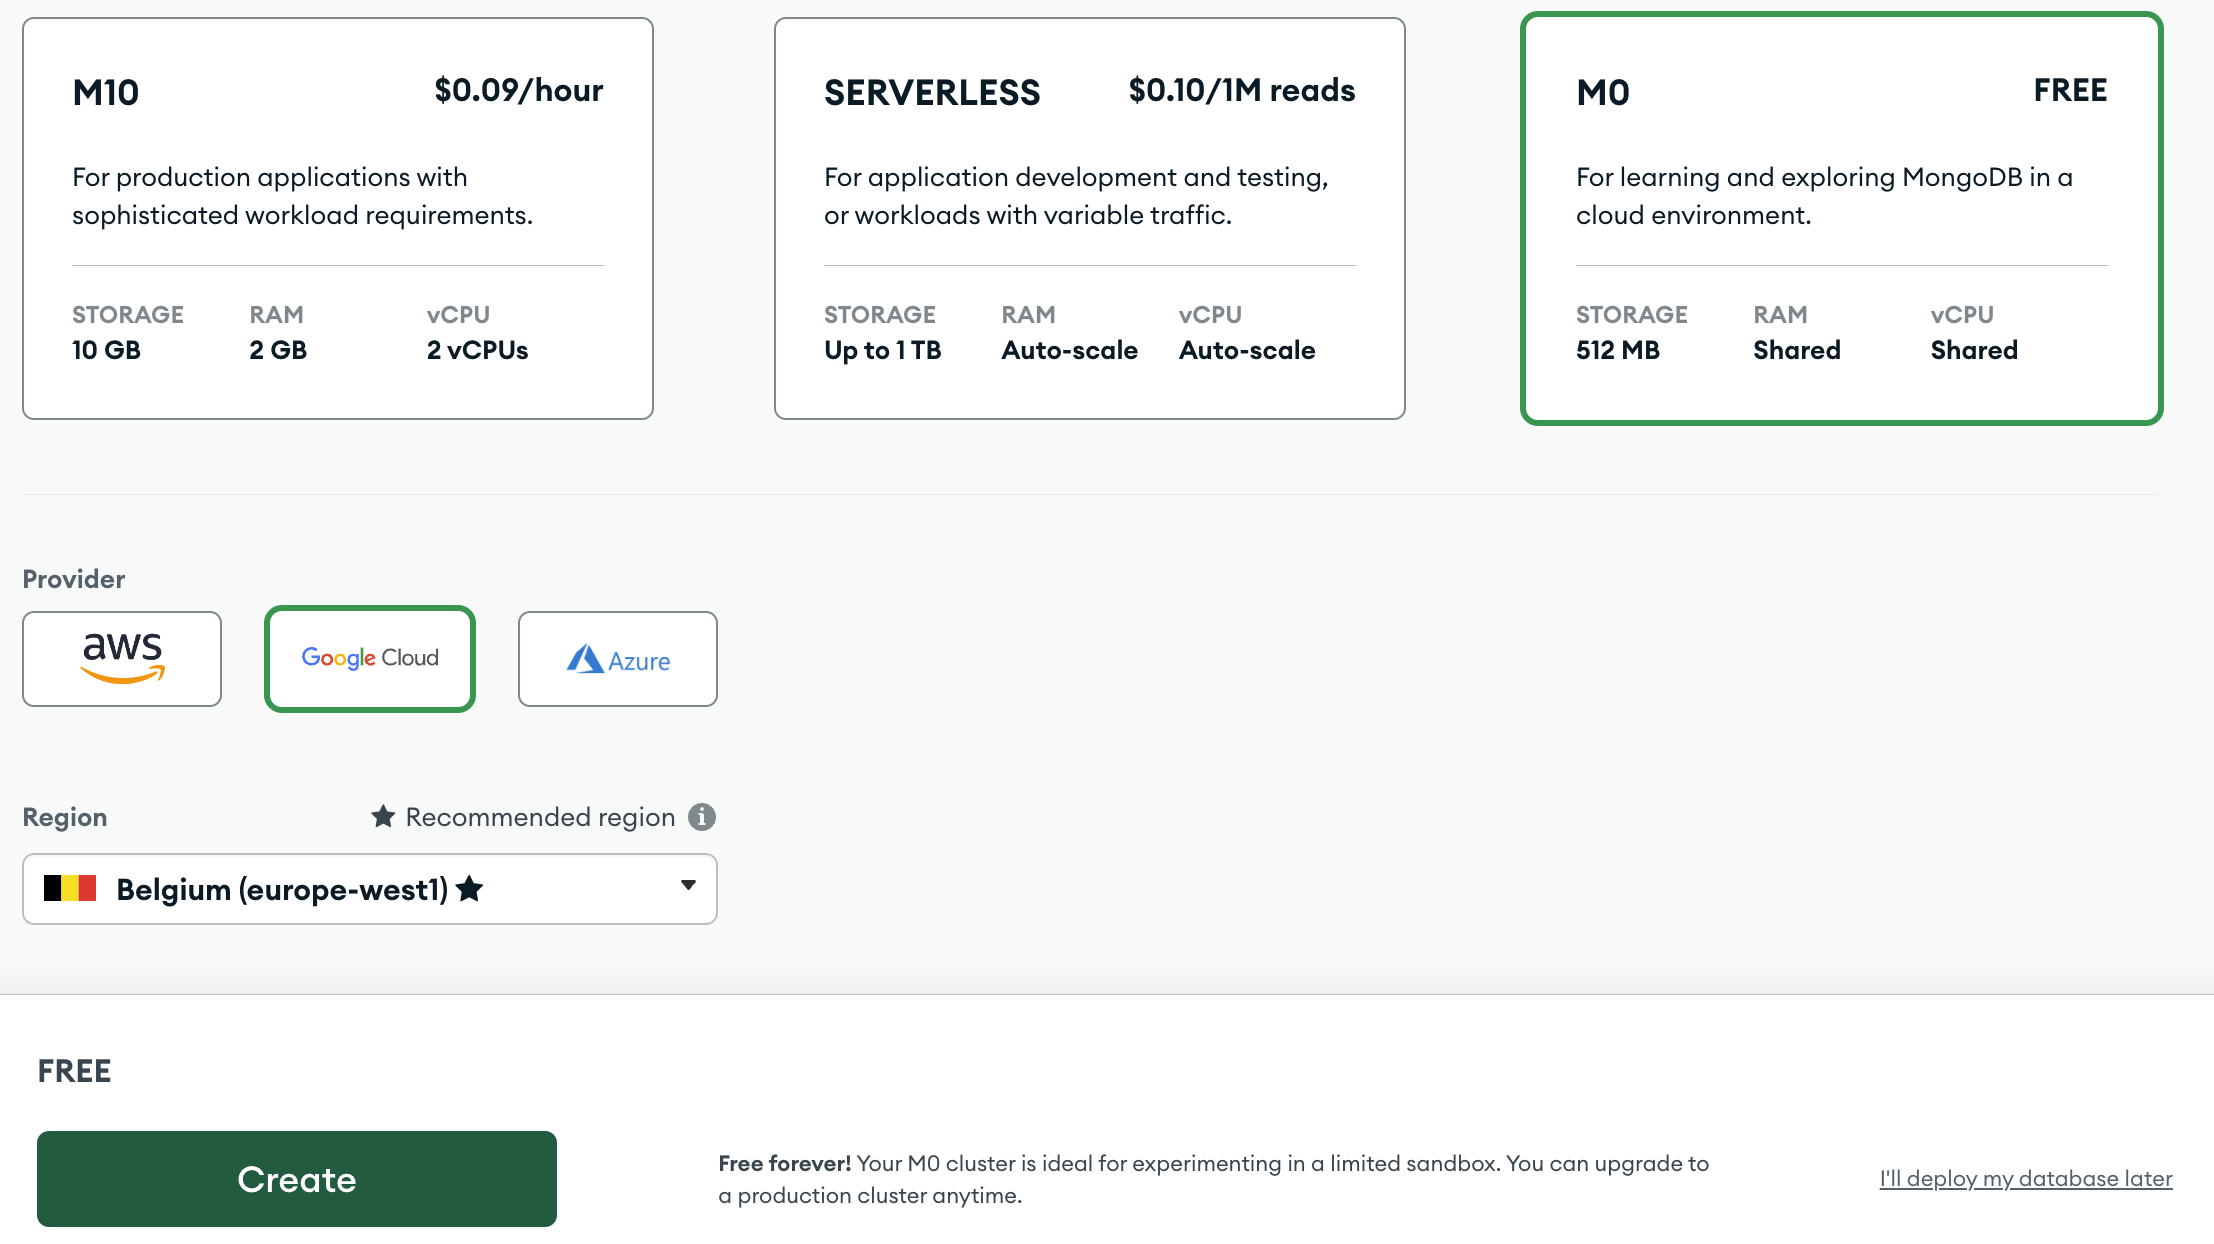
\includegraphics[width=\textwidth]{images/sc01.png}
	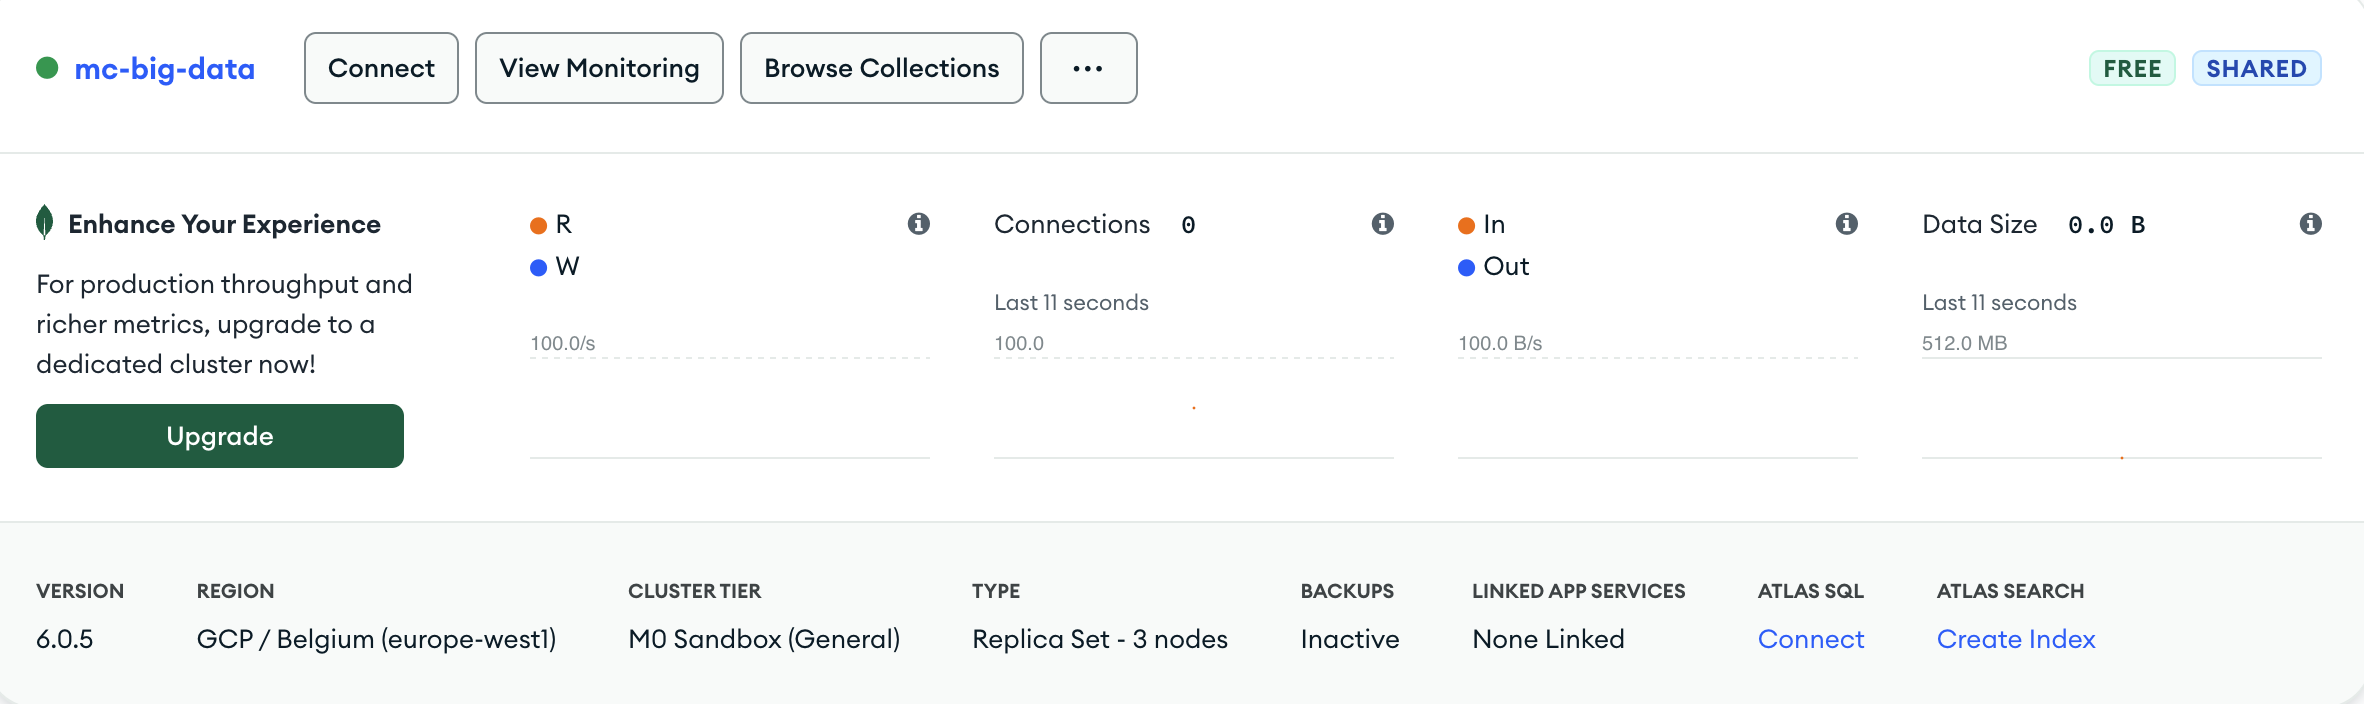
\includegraphics[width=\textwidth]{images/sc02.png}

	\vspace{1cm}

	\noindent \textbf{Enable and configure Data API} \\
	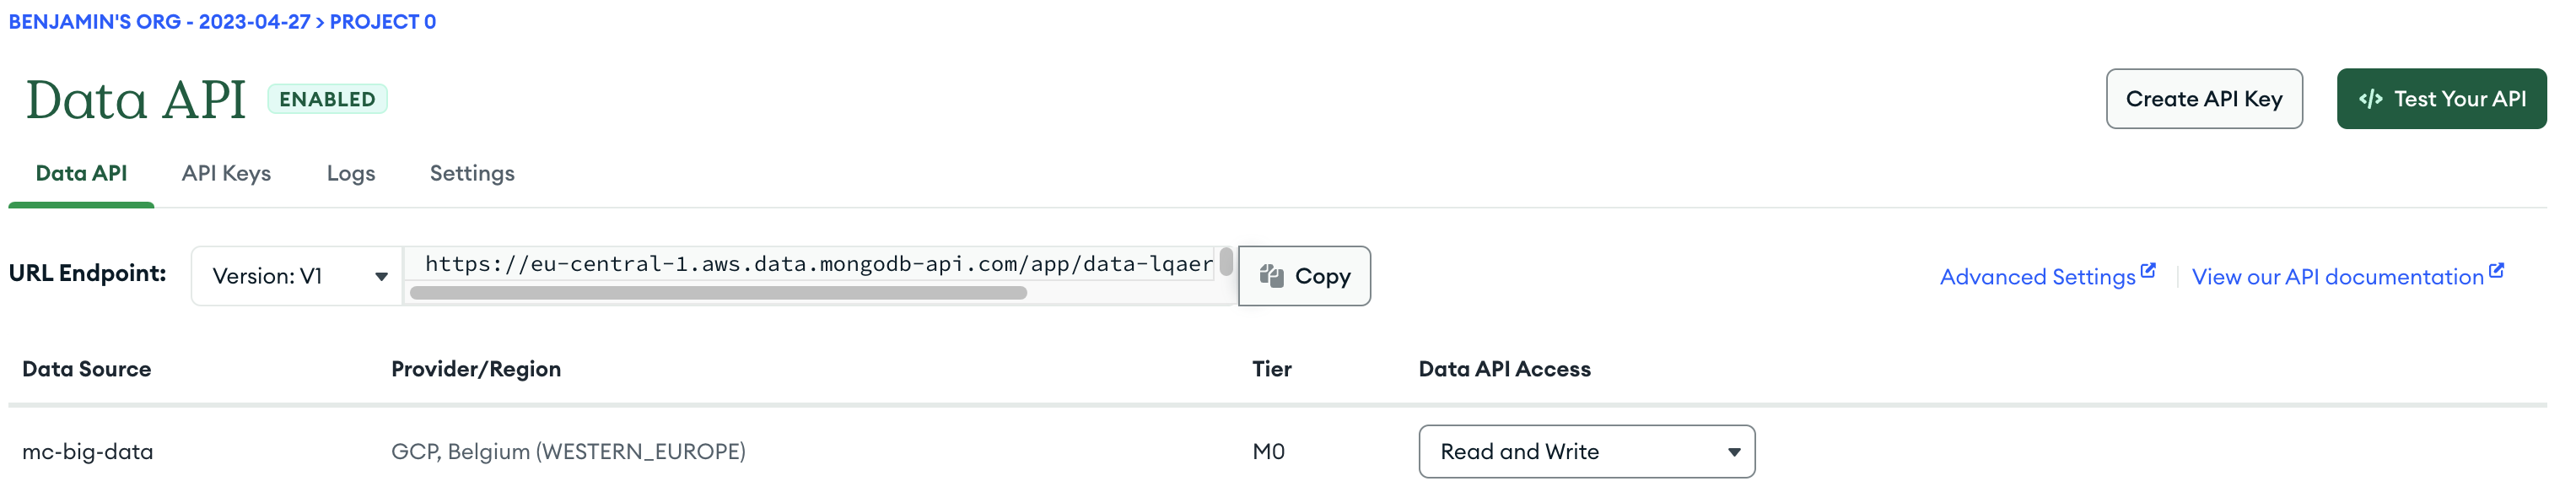
\includegraphics[width=\textwidth]{images/sc03.png}

	\newpage


	\noindent \textbf{Create API Key} \\
	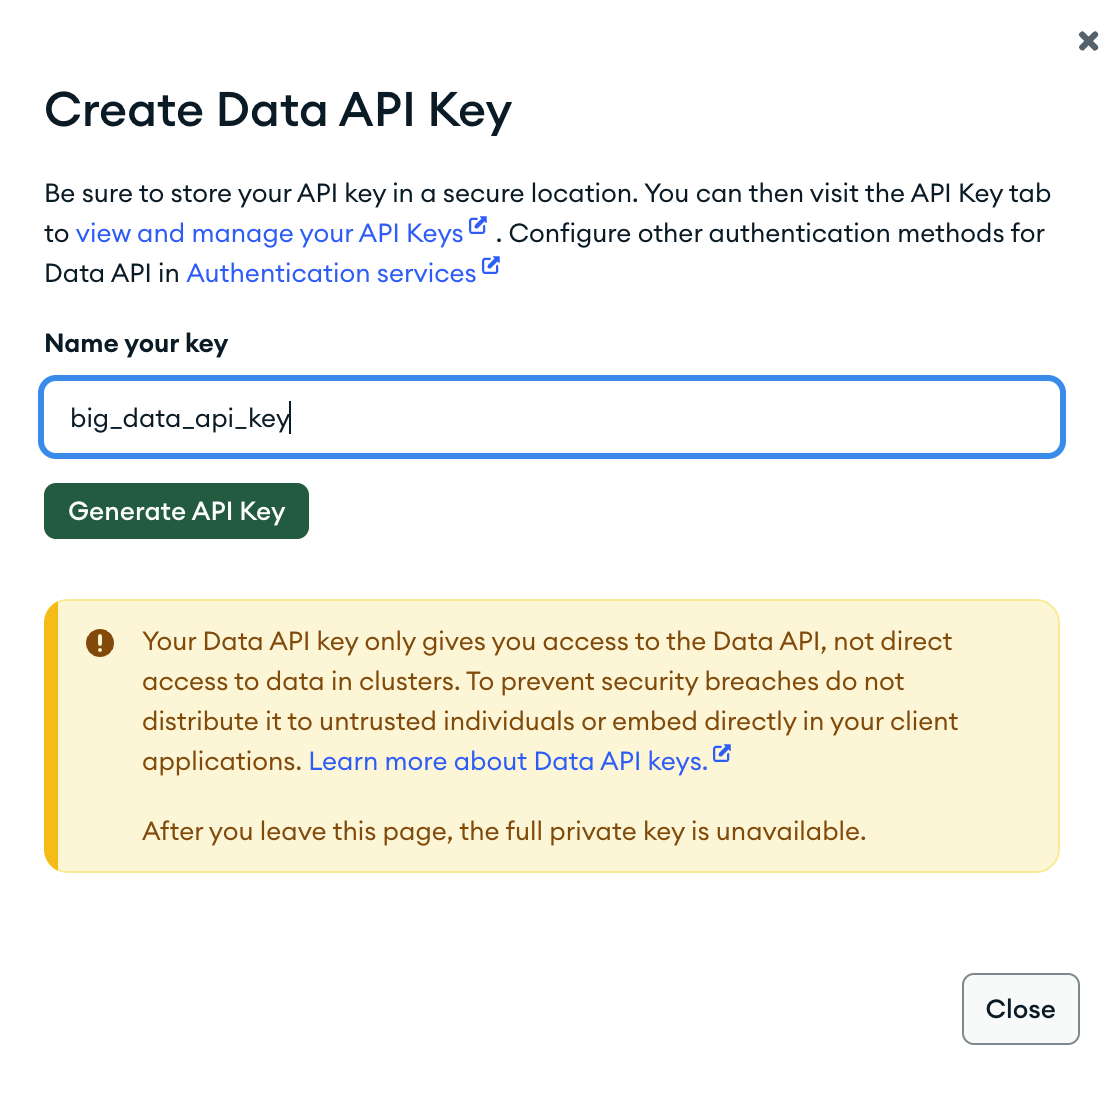
\includegraphics[width=\textwidth]{images/sc04.png}

	\noindent \textbf{Create Environment variables in .zshrc} \\
	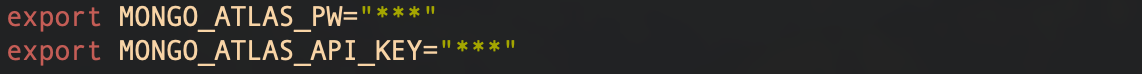
\includegraphics[width=\textwidth]{images/sc05.png}

	\newpage

	\noindent \textbf{Connect using mongo shell} \\
	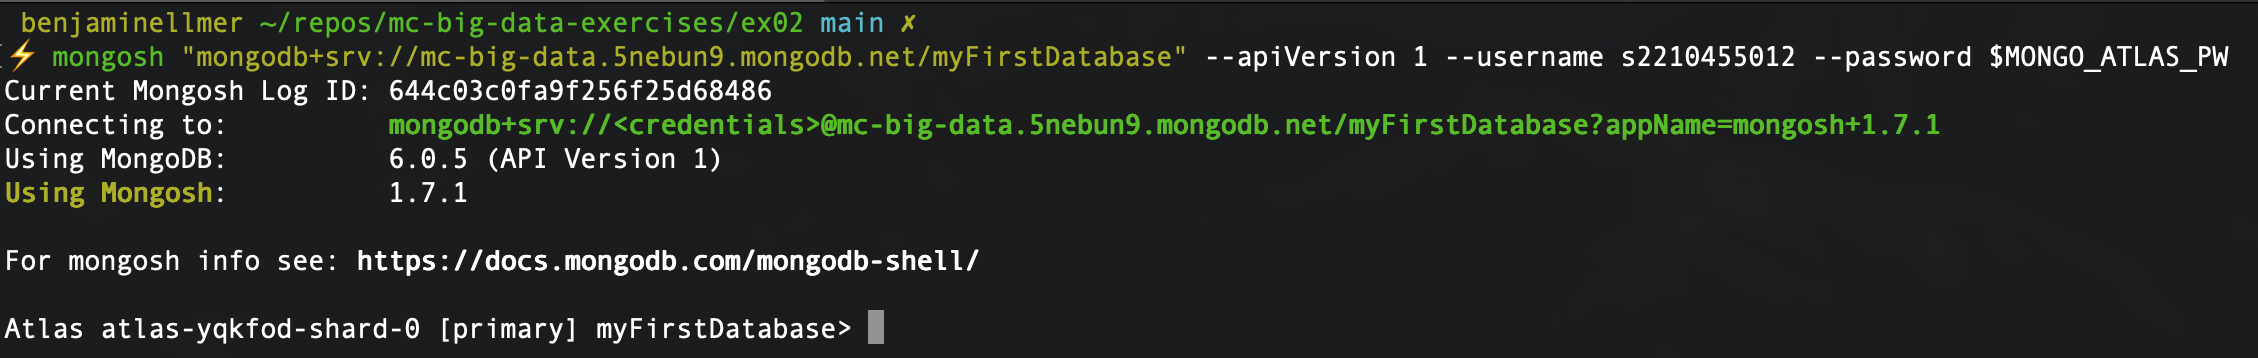
\includegraphics[width=\textwidth]{images/sc06.png}

	\noindent \textbf{Create Database and Sample Data} \\
	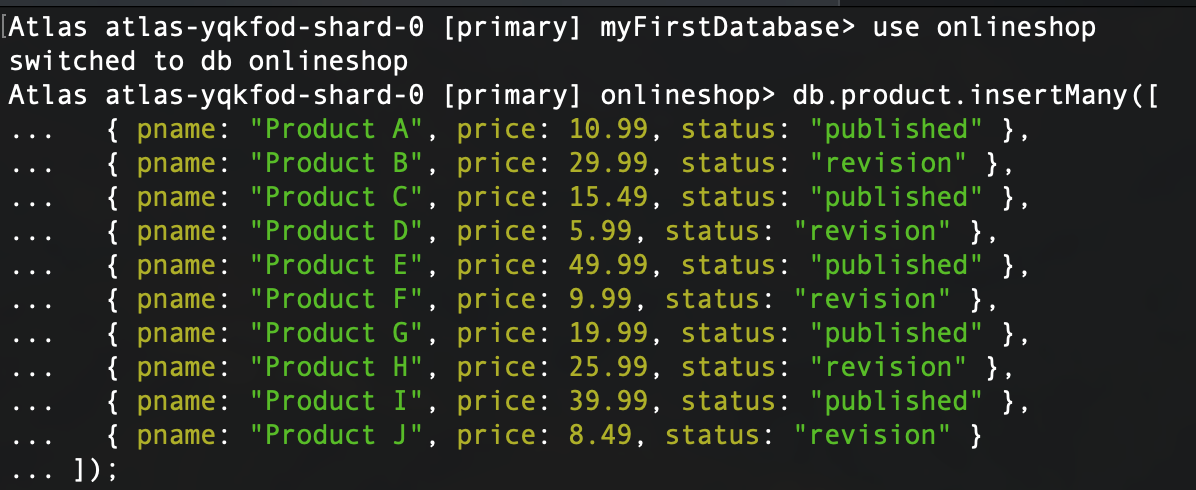
\includegraphics[width=0.9\textwidth]{images/sc07.png} \\
	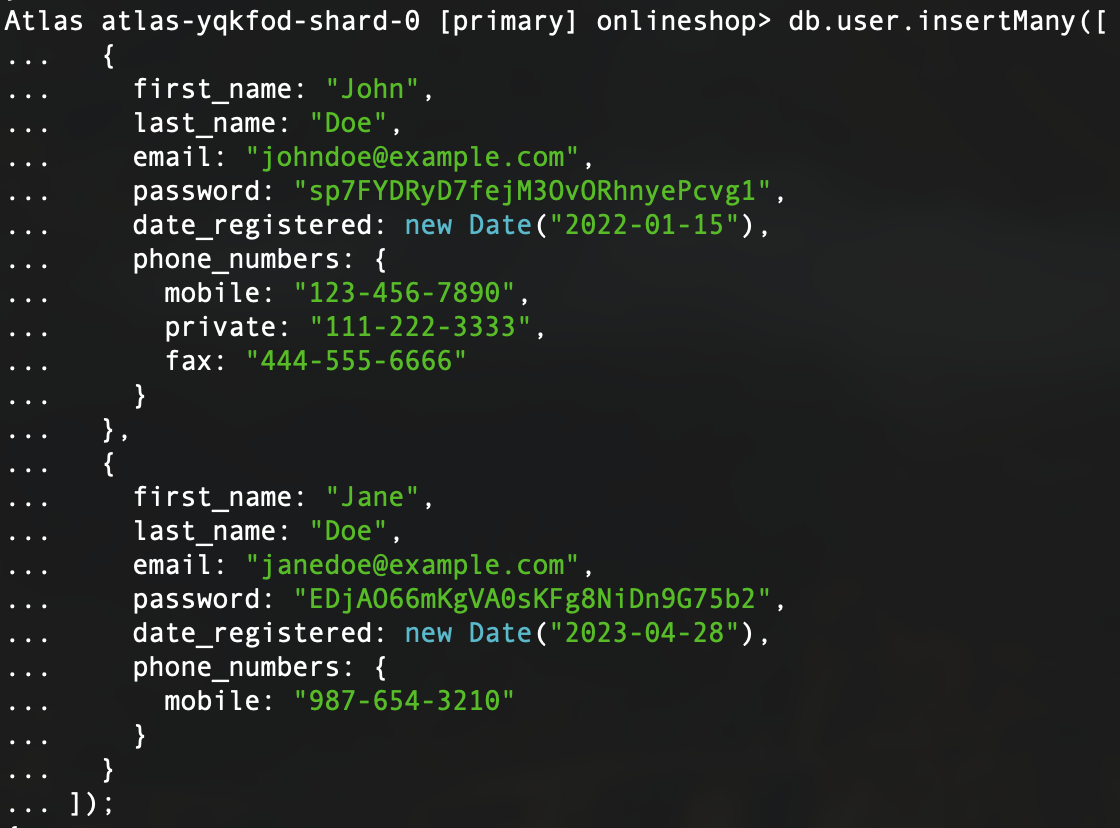
\includegraphics[width=0.9\textwidth]{images/sc08.png} 

	\newpage

	\noindent \textbf{findOne with Data API} \\
	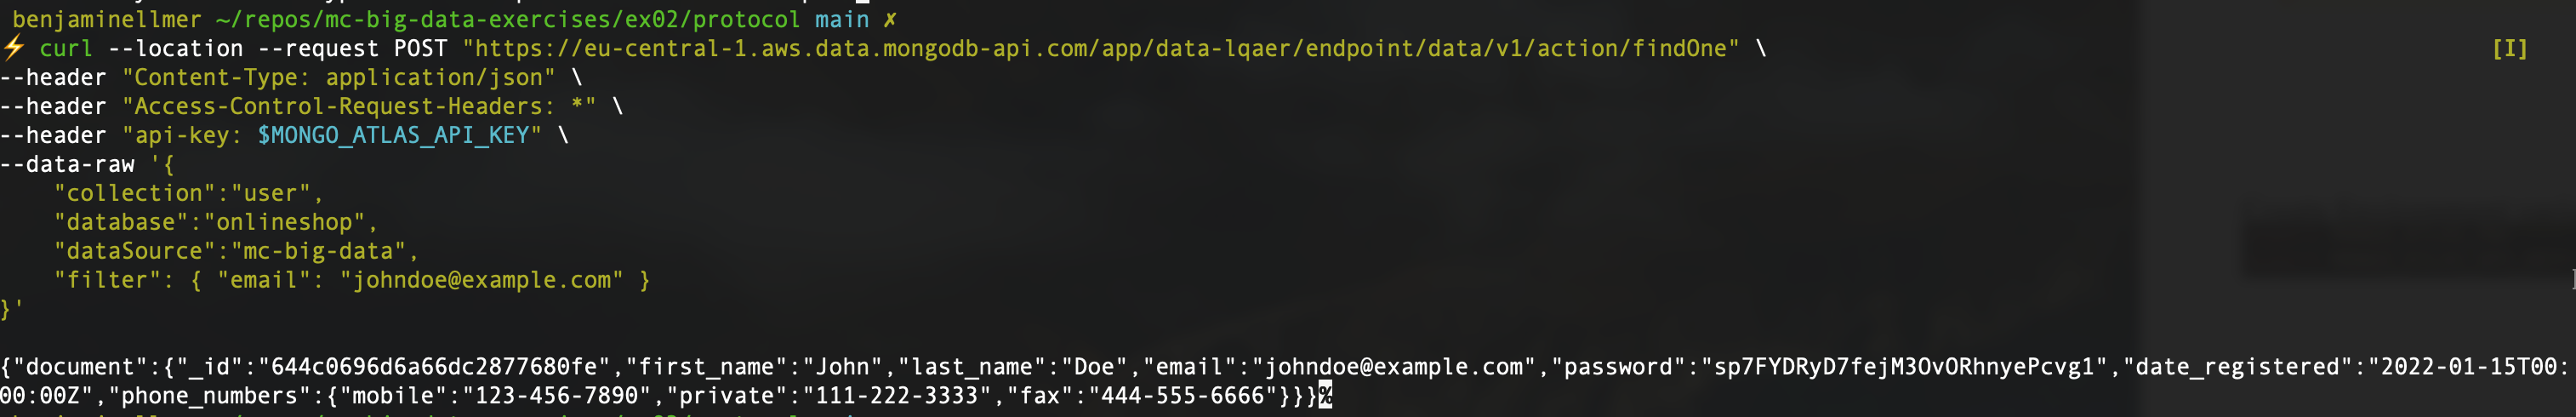
\includegraphics[width=\textwidth]{images/sc09.png}

	\noindent \textbf{findMany with Data API} \\
	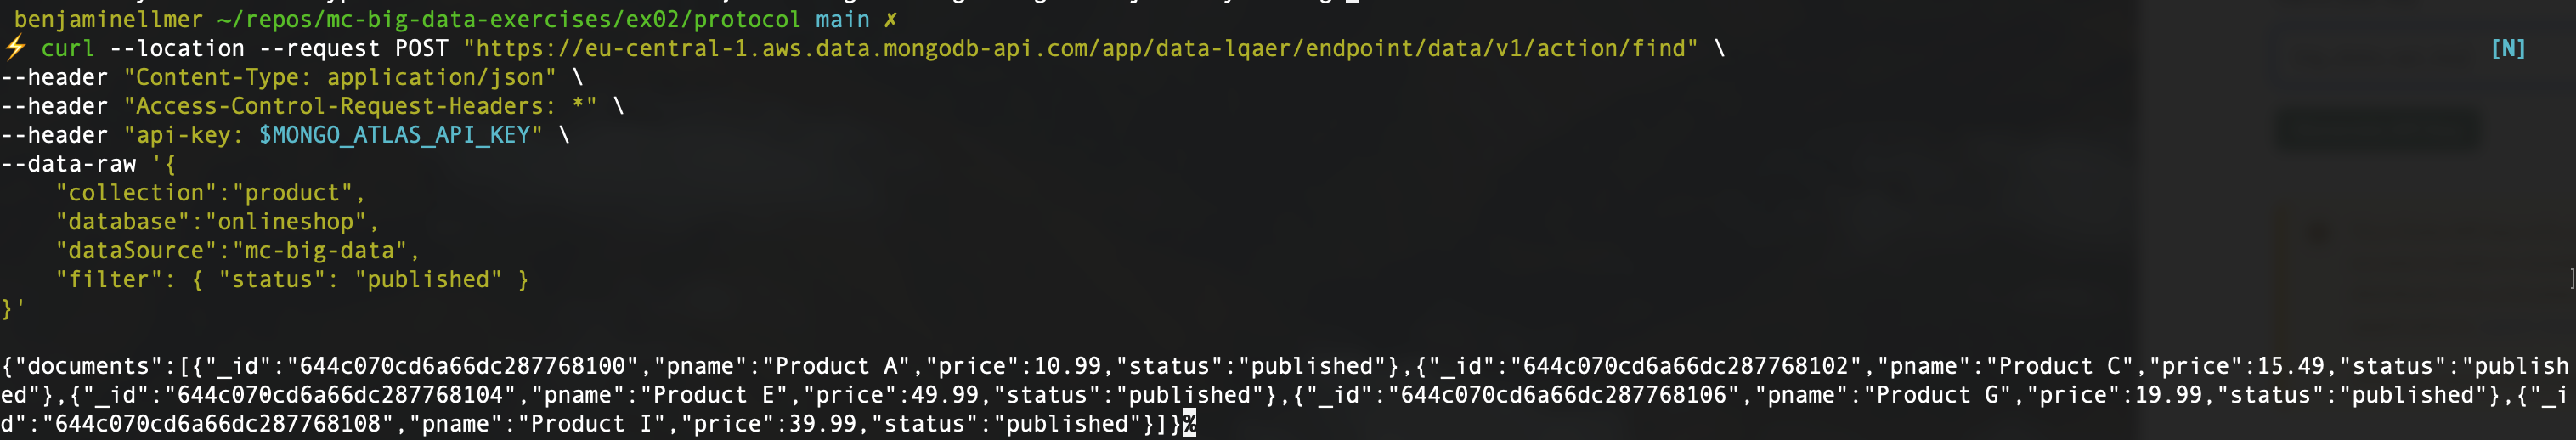
\includegraphics[width=\textwidth]{images/sc10.png} 

	\noindent \textbf{insertOne with Data API} \\
	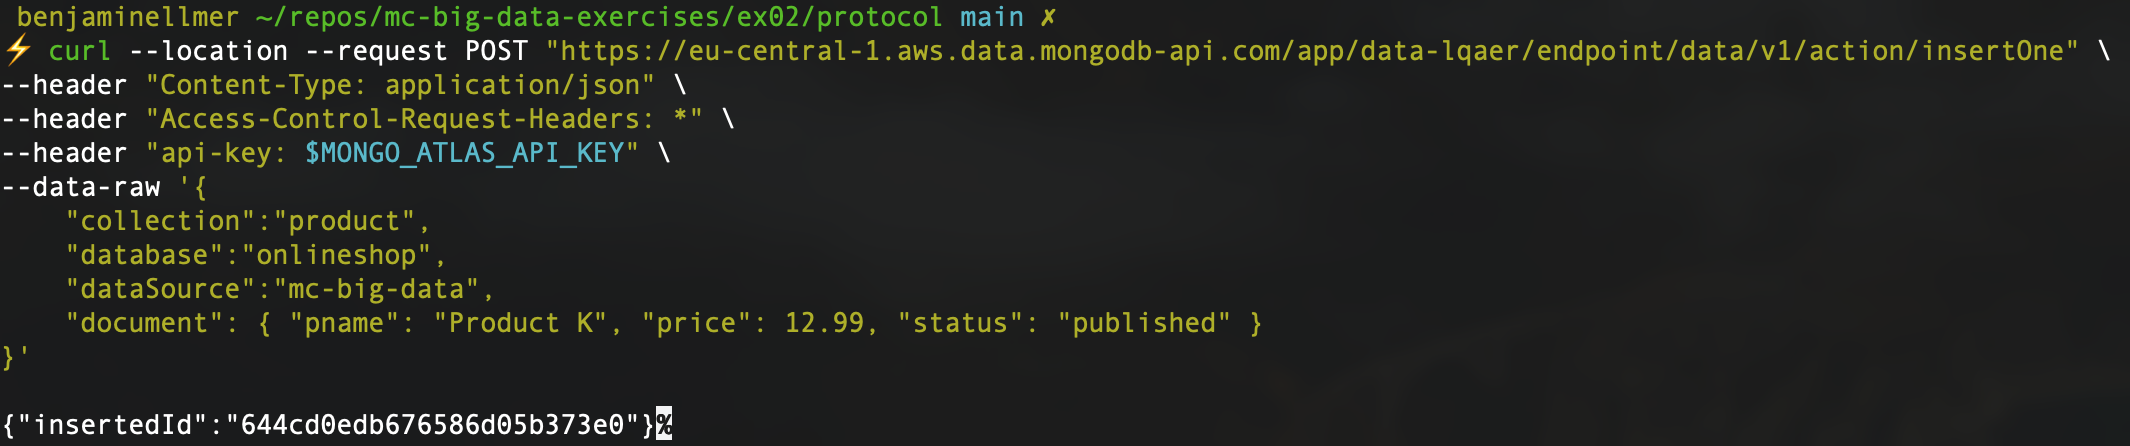
\includegraphics[width=\textwidth]{images/sc11.png} 

	\noindent \textbf{updateOne with Data API} \\
	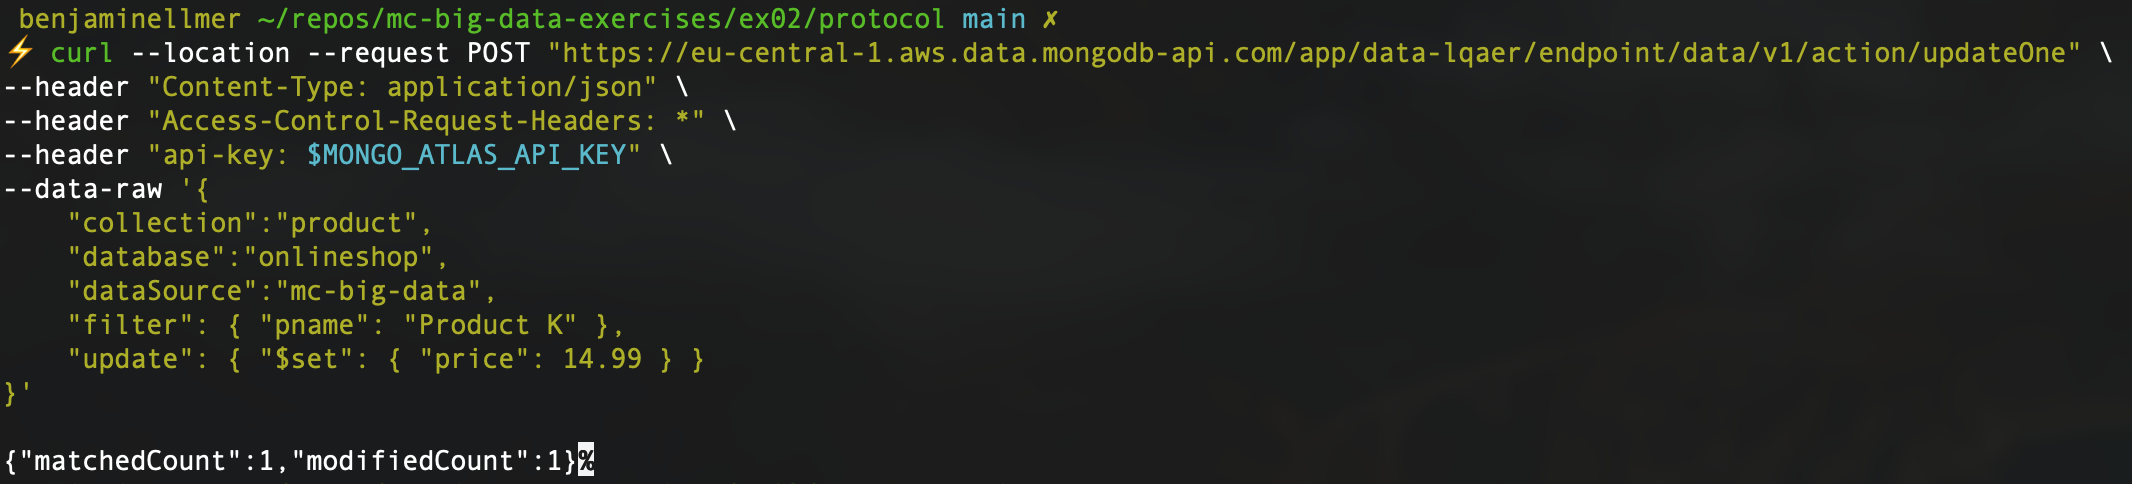
\includegraphics[width=\textwidth]{images/sc12.png} 

	\noindent \textbf{deleteOne with Data API} \\
	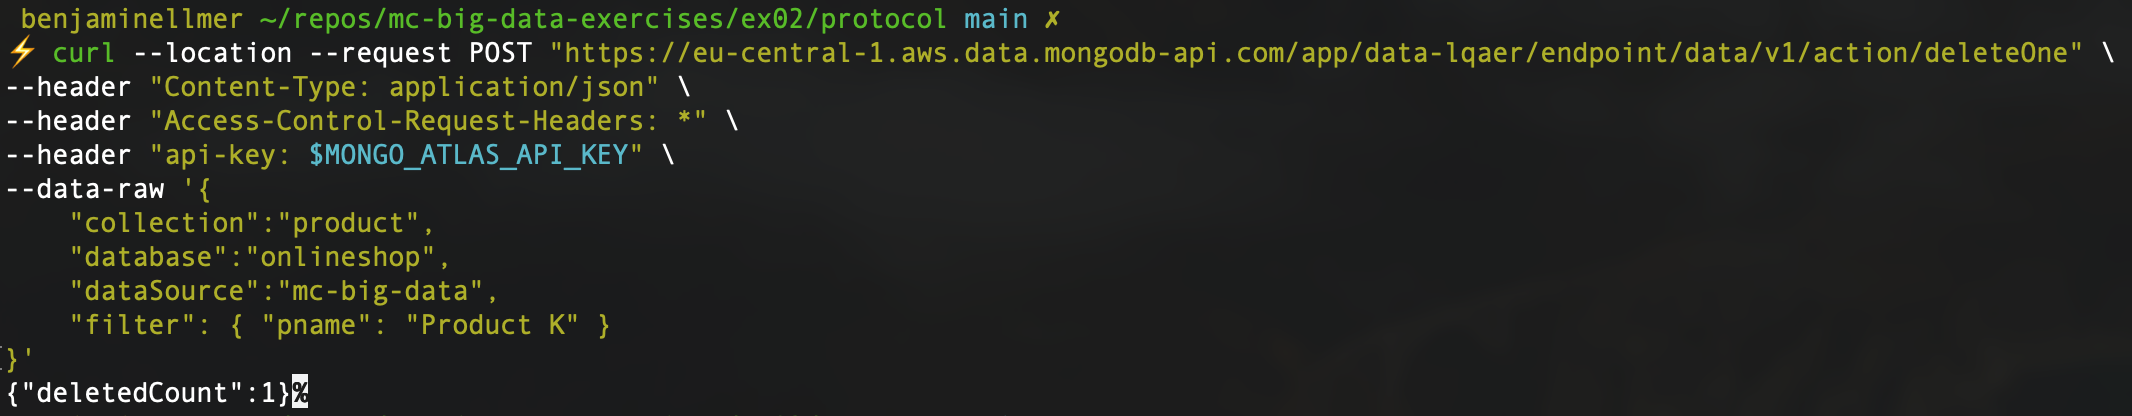
\includegraphics[width=\textwidth]{images/sc13.png} 

	%\noindent \textbf{The pipeline fails because data is already in use} \\
	%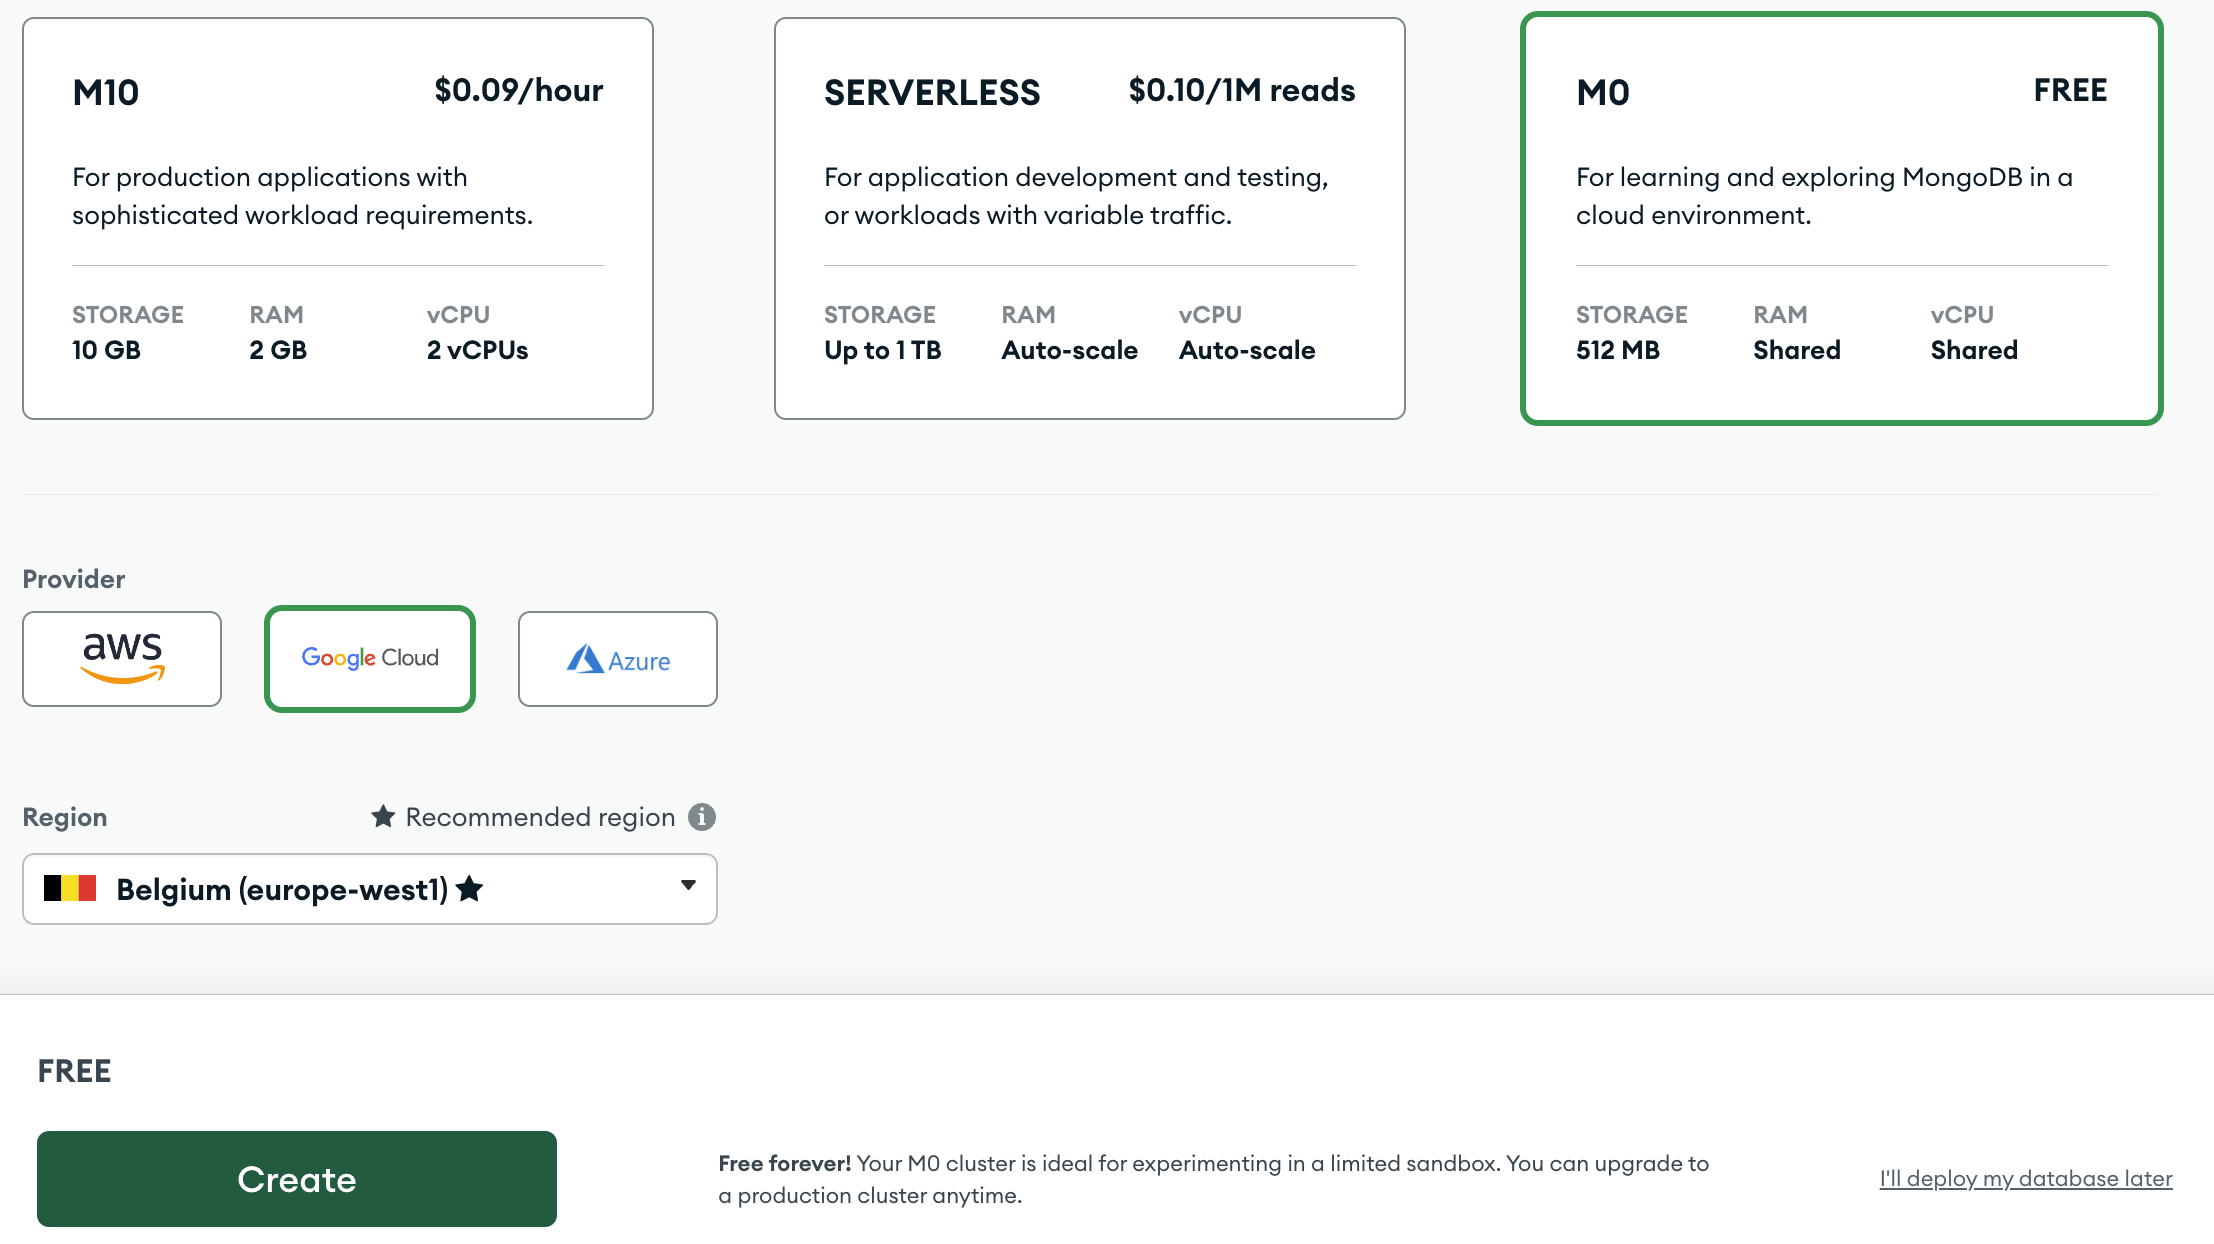
\includegraphics[width=\textwidth]{images/sc01.png} 
	%See \hyperref[listings:pipeline]{pipeline.conf} in appendix for the pipeline 
	%\begin{enumerate}[noitemsep]
		%\item Import the json file using mongoimport
	%\end{enumerate}

	%\newpage
	
	%\section*{Appendix}

	%\subsection*{.env}
	%\label{listings:envs}
	%\lstinputlisting[style=json]{.env}

\end{document}

